\documentclass[a4paper,12pt]{article}
\usepackage[utf8]{vietnam}
\usepackage{hyperref}
\usepackage{graphicx}
\usepackage{xcolor}
\usepackage{subfigure}
\usepackage{float}
\usepackage{caption}
\hypersetup{
	pdfborder = {0 0 0}
}
\title{\textbf{Báo cáo giữa kì \\ Thực hành kiến trúc máy tính}}
\author{Họ tên: Phan Minh Anh Tuấn \\ MSSV: 20205227}
\date{}
\begin{document}
	\maketitle
	\tableofcontents
	\newpage
\section{Bài 6}
\subsection{Đề bài}Given an array of .word elements and the number of elements, write a procedure to find the pair of adjacent elements that has the largest product and return that product. \\ \\
\textbf{MSSV: 20205227} \\
$\Rightarrow$ A: .word 2, 0, 2, 0, 5, 2, 2, 7
\subsection{Ý tưởng} Ban đầu, ta khởi tạo một biến chứa giá trị tích hai phần tử liền kề lớn nhất. Sau đó, ta dùng vòng lặp để duyệt từ đầu đến cuối mảng, tính giá trị tích các cặp phần tử liền kề và cập nhật giá trị cho max.
\begin{figure}[!h]
	\centerline{\fbox{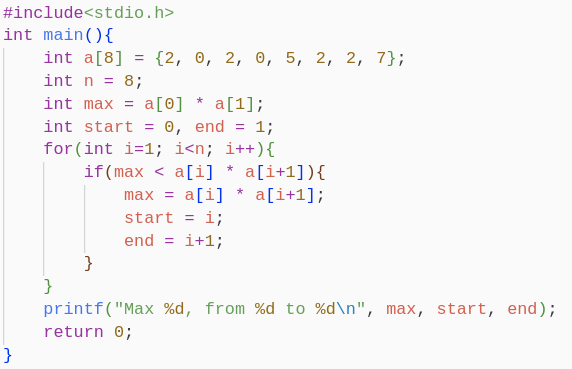
\includegraphics[width=1\textwidth]{bai6/6-c-tuan.png}}}
	\caption{Code C bài tập 6}
	\label{fig:bai6}
\end{figure}
\clearpage
\subsection{Triển khai MIPS}
Ý nghĩa các thanh ghi được sử dụng cố định trong chương trình:
\begin{itemize}
    \item \$s0: Địa chỉ của mảng A
    \item \$s1: Giá trị chỉ số i để chạy vòng lặp
    \item \$s2: n-2, với n là số phần tử của mảng
    \item \$s3: Bước nhảy của vòng lặp
    \item \$s4: Giá trị tích cặp phần tử liền kề lớn nhất trong mảng
    \item \$a1:	Giá trị phần tử thứ nhất trong cặp phần tử đang xét	
    \item \$a2:	Giá trị phần tử thứ hai trong cặp phần tử đang xét
    \item \$t3: Thanh ghi lưu lại giá trị phần tử thứ nhất trong cặp phần tử đang xét
    \item \$t4: Thanh ghi lưu lại giá trị phần tử thứ hai trong cặp phần tử đang xét
\end{itemize}
Các thanh ghi còn lại có ý nghĩa khác nhau ở mỗi hàm trong chương trình.
\begin{figure}[!h]
	\centerline{\fbox{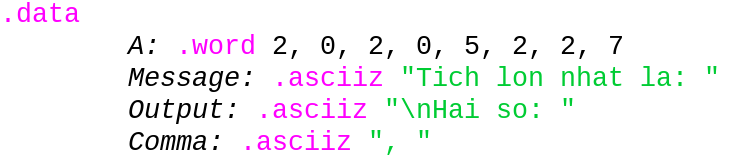
\includegraphics[width=1\textwidth]{bai6/data-6-tuan.png}}}
	\caption*{\textbf{Bước 1:} Khởi tạo giá trị ban đầu cho mảng, tạo các string in ra màn hình.}
	\label{fig:data6}
\end{figure}
\clearpage
\begin{figure}[!h]
	\centerline{\fbox{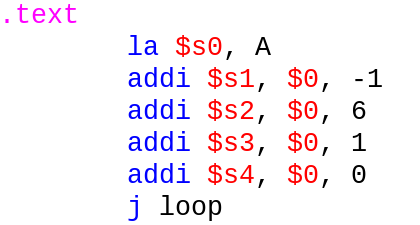
\includegraphics[width=0.65\textwidth]{bai6/text6-1.png}}}
	\caption*{\textbf{Bước 2:} Khởi tạo, gán giá trị}
	\label{fig:data6}
\end{figure}
\noindent
\textbf{Trong đó: }
\begin{itemize}
    \item \$s1: Giá trị ban đầu của chỉ số i = -1
    \item \$s2: n-2, với n là số phần tử của mảng, cụ thể ở đây mảng có 8 phần tử nên \$s2 = 6
\end{itemize}
% \clearpage
\begin{figure}[!h]
	\centerline{\fbox{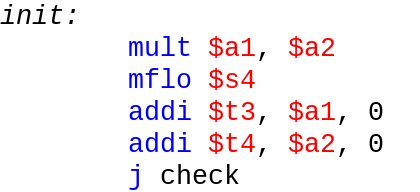
\includegraphics[width=0.65\textwidth]{bai6/text6-2.png}}}
	\caption*{\textbf{Bước 3:} Khởi tạo giá trị tích cặp phần tử liền kề lớn nhất}
	\label{fig:data6}
\end{figure}
\noindent
\textbf{Trong đó: }
\begin{itemize}
    \item \$a1:	Giá trị phần tử thứ nhất trong mảng	
    \item \$a2:	Giá trị phần tử thứ hai trong mảng
    \item \$s4: Giá trị tích lớn nhất tính đến hiện tại
\end{itemize}
\noindent
\textbf{Giải thích: }Hàm \textbf{init} thực hiện tính tích hai phần tử đầu tiên của mảng và lưu vào thanh ghi \$s4, đây được coi là giá trị tích lớn nhất tính đến hiện tại. Sau đó, hàm thực hiện lưu lại giá trị của hai phần tử đầu tiên đó vào thanh ghi \$t3 và \$t4, đó là kết quả cặp phần tử cần tìm.
\clearpage
\begin{figure}[!h]
	\centerline{\fbox{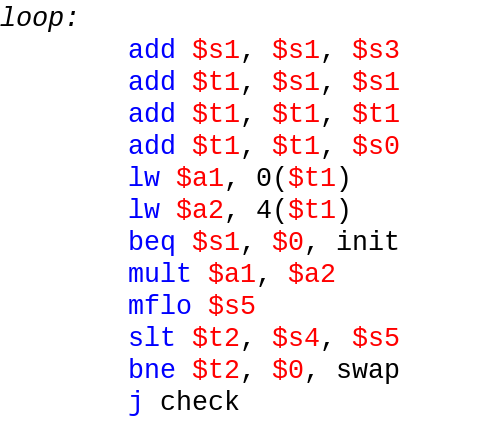
\includegraphics[width=0.8\textwidth]{bai6/text6-3.png}}}
	\caption*{\textbf{Bước 4:} Vòng lặp tìm giá trị tích hai phần tử liền kề lớn nhất trong mảng}
	\label{fig:data6}
\end{figure}
\noindent
\textbf{Trong đó: }
\begin{itemize}
    \item \$s5:	Giá trị tích của cặp phần tử đang xét
    \item \$t1: Địa chỉ của phần tử thứ nhất trong cặp phần tử đang xét
    \item \$t2: Nếu giá trị tích lớn nhất tính đến hiện tại nhỏ hơn tích của cặp phần tử đang xét thì \$t2 = 1, ngược lại \$t2 = 0
\end{itemize}
\noindent
\textbf{Giải thích: }Đầu tiên, ta thực hiện tính địa chỉ của phần tử A[i] của mảng bằng phương pháp chỉ số: \$t1 = địa chỉ A[i] = 4.(i + step) = 2.2.(\$s1 +\$s3). Sau đó ta load giá trị của A[i] và A[i+1] lần lượt vào \$a1 và \$a2. Kiểm tra đây có phải là lần lặp đầu tiên không bằng cách so sánh chỉ số i có bằng 0 hay không, nếu không thực hiện so sánh tích \$a1 và \$a2 hiện thời với \$s4 (tích lớn nhất hiện tại) để cập nhật \$s4, nếu là lần lặp đầu tiên, thực hiện hàm \textbf{init}.
\clearpage
\begin{figure}[!h]
	\centerline{\fbox{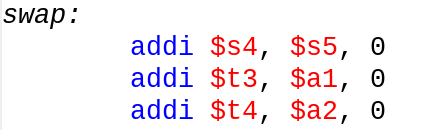
\includegraphics[width=0.75\textwidth]{bai6/text6-4.png}}}
	\caption*{\textbf{Bước 5:} Cập nhật giá trị tích hai phần tử liền kề lớn nhất của mảng}
	\label{fig:data6}
\end{figure}
\noindent
\textbf{Trong đó: }
\begin{itemize}
    \item \$s5:	Giá trị tích của cặp phần tử đang xét
\end{itemize}
\noindent
\textbf{Giải thích: }Hàm \textbf{swap} thực hiện đổi chỗ hai giá trị: giá trị tích lớn nhất tính đến hiện tại (\$s4) và giá trị tích hai phần tử liền kề đang xét (\$s5), nếu \$s4 < \$s5. Cách thực hiện như sau: Gán giá trị \$s4 = giá trị \$s5. Sau đó, ta lưu lại vết 2 phần tử có tích lớn nhất vào \$t3 và \$t4.
% \clearpage
\begin{figure}[!h]
	\centerline{\fbox{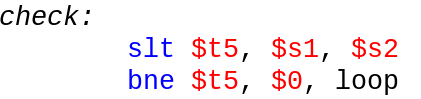
\includegraphics[width=0.75\textwidth]{bai6/text6-5.png}}}
	\caption*{\textbf{Bước 6:} Kiểm tra điều kiện vòng lặp}
	\label{fig:data6}
\end{figure}
\\
\noindent
\textbf{Trong đó: }
\begin{itemize}
    \item \$s1: Giá trị của chỉ số i
    \item \$s2: n-2, với n là số phần tử của mảng
    \item \$t5: Nếu i < $n-2$ thì \$t5 = 1, ngược lại \$t5 = 0
\end{itemize}
\noindent
\textbf{Giải thích: }Vì mỗi lần duyệt ta xét từng cặp hai phần tử nên ta chỉ cần thực hiện vòng lặp đến cặp phần tử A[n-2] và A[n-1]. Do đó, ta kiểm tra điều kiện chỉ số i < n-2, khi i tăng đến bằng n-2 thì điều kiện này sai, \$t5 = 0 và vòng lặp được dừng lại.
\clearpage
\subsection{Kết quả}
\begin{figure}[!h]
	\centerline{\fbox{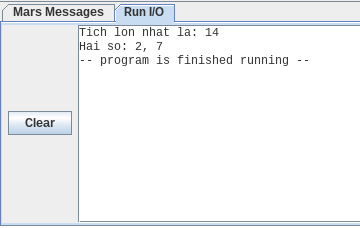
\includegraphics[width=1\textwidth]{bai6/kq-6-tuan.png}}}
	\caption{Kết quả đoạn code trên}
	\label{fig:data6}
\end{figure}
\noindent
\textbf{Nhận xét: }Chương trình tìm ra tích cặp phần tử liền kề lớn nhất là 14, là tích của cặp phần tử 2 và 7. Kết quả này là chính xác.
\clearpage
\section{Bài 1}
\subsection{Đề bài}
Create a program to input a text line from the keyboard and test if it is a
palindrome. For example: “abc121cba” is a palindrome. Store all palindromes which
the user typed into the memory, to make sure that the user does not duplicate
palindromes.
\subsection{Ý tưởng}
Chương trình thực hiện lần lượt các hàm tương ứng với các chức năng theo yêu cầu đề bài như sau:
\begin{itemize}
    \item \textbf{getString}: cho phép người dùng nhập một xâu từ bàn phím thông qua một hộp thoại
    \item \textbf{getLength}: tìm độ dài của xâu vừa nhập, chuẩn hóa xâu bằng cách xóa bỏ ký tự xuống dòng và trả về chỉ số phần tử cuối cùng của xâu.
    \item \textbf{isTooLongString}: giới hạn số ký tự nhập vào (nhỏ hơn 50 ký tự). Nếu thỏa mãn độ dài cho phép thì đi đến hàm \textbf{isStoredInMemony}. Nếu độ dài xâu lớn hơn 50 ký tự (tính cả ký tự kết thúc xâu) thì báo lỗi và yêu cầu nhập lại. 
    \item \textbf{isStoredInMemory}: kiểm tra xâu vừa nhập đã được lưu trong bộ nhớ chưa. Nếu đã lưu trong bộ nhớ thì hiển nhiên xâu vừa nhập là đối xứng, thông báo cho người dùng. Nếu không thì đi đến kiểm tra xâu đối xứng.
    \item \textbf{checkPalindrome}: kiểm tra xâu vừa nhập có phải là xâu đối xứng hay không. Nếu có thì lưu vào bộ nhớ, nếu không thì thông báo cho người dùng.
    \item \textbf{storeStringInMemory}: lưu xâu đối xứng vừa kiểm tra được vào bộ nhớ. Nếu bộ nhớ đầy thì không lưu vào.
\end{itemize}
Ngoài ra, chương trình bao gồm các hàm để in thông báo ra màn hình và xác nhận thực hiện chương trình tiếp hay không thông qua các hộp thoại.
\clearpage
\subsection{Triển khai MIPS}
Ý nghĩa các thanh ghi được sử dụng cố định trong chương trình:
\begin{itemize}
    \item \$s0: Địa chỉ của xâu nhập vào (Input)
    \item \$s1: Độ dài của xâu nhập vào 
    \item \$s2: Địa chỉ của mảng lưu các xâu đã được nhập vào mà đối xứng (StringList)
\end{itemize}
Các thanh ghi còn lại có ý nghĩa khác nhau ở mỗi hàm trong chương trình.
\subsubsection{Khởi tạo}
\begin{figure}[!h]
	\centerline{\fbox{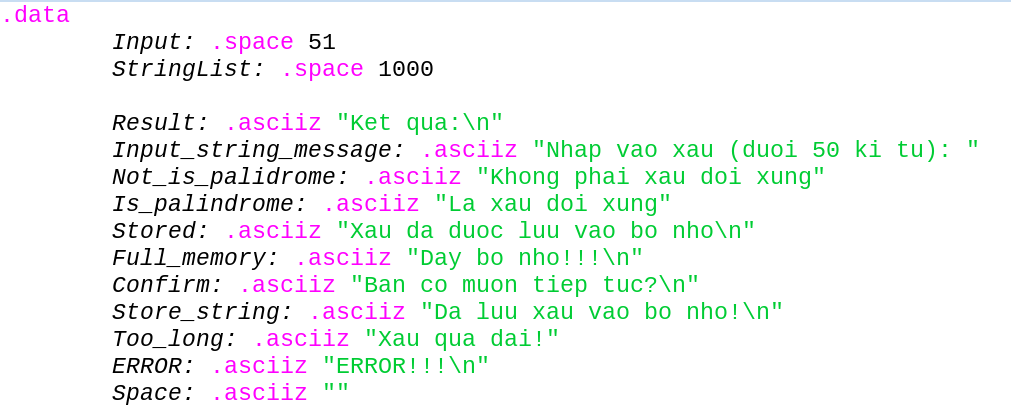
\includegraphics[width=1\textwidth]{bai1/1-init.png}}}
	\caption{Các xâu khởi tạo để in ra màn hình}
	\label{fig:bai6}
\end{figure}
\clearpage
\begin{figure}[!h]
	\centerline{\fbox{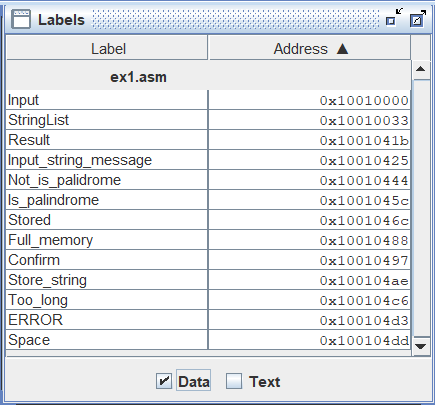
\includegraphics[width=0.7\textwidth]{bai1/labels-window.png}}}
	\caption{Tên các biến và địa chỉ của chúng trong bộ nhớ}
	\label{fig:bai1}
\end{figure}
% \clearpage
\subsubsection{Input}
\begin{figure}[!h]
	\centerline{\fbox{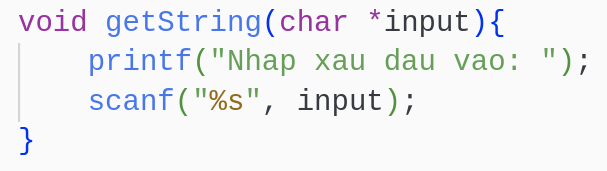
\includegraphics[width=0.72\textwidth]{bai1/1-getstring-c.png}}}
	\label{fig:bai6}
\end{figure}
\begin{figure}[!h]
	\centerline{\fbox{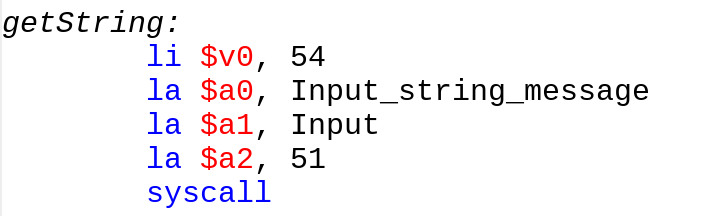
\includegraphics[width=0.72\textwidth]{bai1/1-input.png}}}
	\caption{Nhập giá trị xâu đầu vào}
	\label{fig:bai6}
\end{figure}
\noindent
\textbf{Trong đó: }
\begin{itemize}
    \item \$v0 = 54: Mode InputDialogString (Hiển thị hộp thoại thông báo để đọc một xâu nhập vào từ bàn phím).
    \item \$a0: Địa chỉ thông báo hiện lên màn hình.
    \item \$a1: Lưu địa chỉ xâu nhập vào.
    \item \$a2: Số ký tự tối đa đọc vào.
\end{itemize}
%!!!!!!!!!!!!!!!!!!!!!!!!!!!!!!!!!!!!!!!!!!!!!!!!!!!!!!!!!!!!!!!
\textbf{Kết quả trả về:} Một xâu dài tối đa 50 ký tự được lưu vào địa chỉ biến Input trong bộ nhớ. Xâu Input được lưu vào bộ nhớ bắt đầu từ địa chỉ 0x10010000, mỗi ký tự được lưu bằng 1 byte, nằm liên tiếp nhau trong bộ nhớ. Lúc này, xâu vẫn bao gồm ký tự xuống dòng ở trước ký tự kết thúc xâu.
\begin{figure}[!h]
	\centerline{\fbox{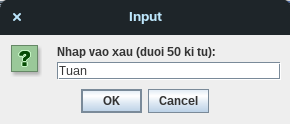
\includegraphics[width=0.75\textwidth]{bai1/T01-hop-thoai-input.png}}}
	\caption{Ví dụ nhập một xâu không đối xứng}
	\label{fig:bai6}
\end{figure}
\begin{figure}[!h]
	\centerline{\fbox{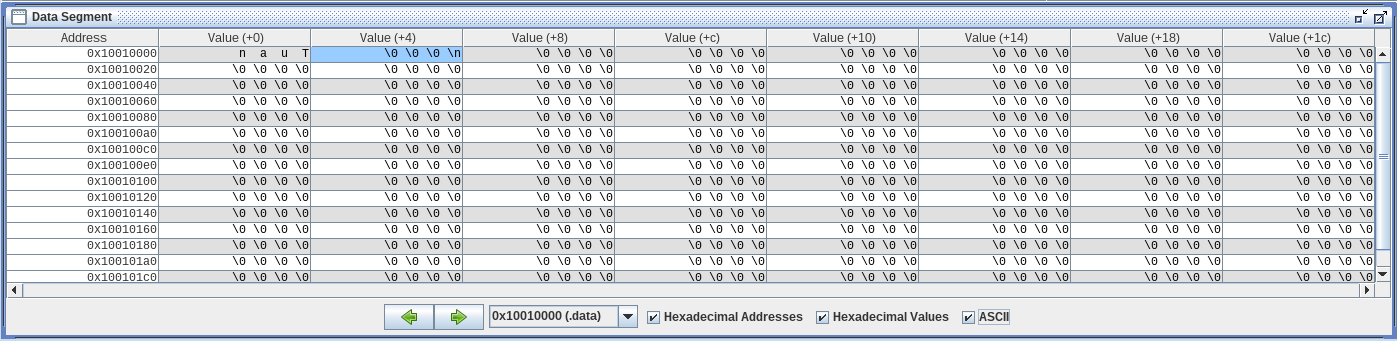
\includegraphics[width=1\textwidth]{bai1/T02-data-segment-input.png}}}
	\caption{Cửa sổ Datasegment sau khi nhập xâu trên}
	\label{fig:bai6}
\end{figure}
\begin{figure}[!h]
	\centerline{\fbox{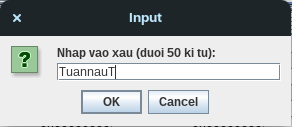
\includegraphics[width=0.75\textwidth]{bai1/T08-hop-thoai-input-2.png}}}
	\caption{Ví dụ nhập một xâu đối xứng}
	\label{fig:bai6}
\end{figure}
\begin{figure}[!h]
	\centerline{\fbox{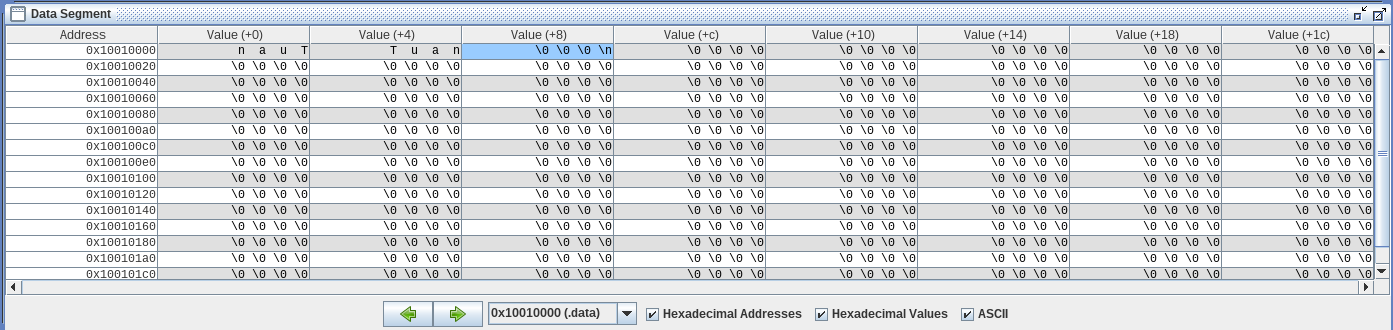
\includegraphics[width=1\textwidth]{bai1/T09-data-segment-input-2.png}}}
	\caption{Cửa sổ Datasegment sau khi nhập xâu trên}
	\label{fig:bai6}
\end{figure}
\clearpage
\subsubsection{getLength}
\begin{figure}[!h]
	\centerline{\fbox{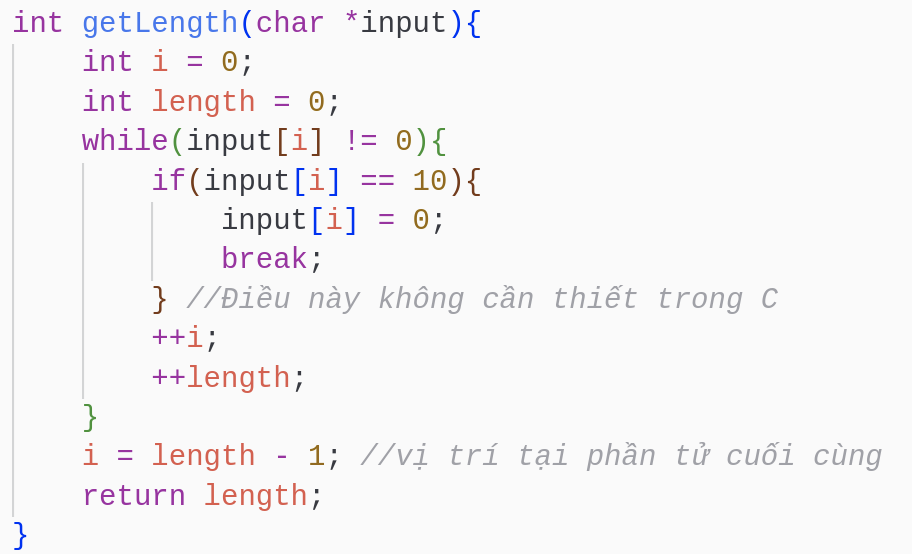
\includegraphics[width=0.85\textwidth]{bai1/1-getlength-c.png}}}
	\label{fig:bai6}
\end{figure}
\begin{figure}[!h]
	\centerline{\fbox{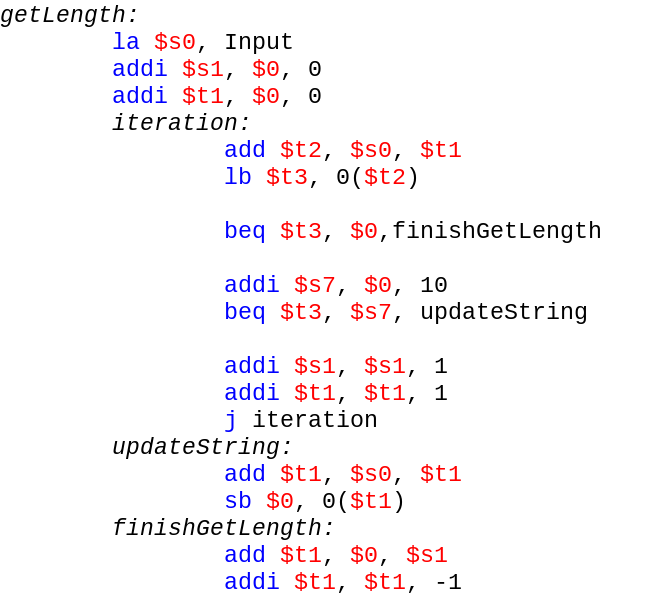
\includegraphics[width=0.75\textwidth]{bai1/1-getlength.png}}}
	\caption{Lấy độ dài xâu đầu vào}
	\label{fig:bai6}
\end{figure}
\clearpage
\noindent
\textbf{Trong đó: }
\begin{itemize}
    \item \$t1: Chỉ số i, dùng để chạy đến cuối xâu Input và lưu lại chỉ số của kí tự cuối cùng (tính từ 0).
    \item \$t2: Địa chỉ của phần tử thứ i trong xâu Input.
    \item \$t3: Giá trị của phần tử thứ i trong xâu Input.
    \item \$s7: Giá trị của ký tự xuống dòng trong bảng mã ASCII (10).
\end{itemize}
\textbf{Giải thích:}
Tạo một vòng lặp (iteration) đếm số ký tự của xâu cho đến khi gặp kí tự kết thúc xâu thì dừng lại và cập nhật chỉ số của ký tự cuối cùng (finishGetLength). Nếu gặp kí tự xuống dòng (mã ASCII = 10) thì gán nó giá trị = 0 (updateString). \\
\textbf{Kết quả trả về:} Sau khi thực hiện hàm getLength, chương trình đã đếm được độ dài của xâu "Tuan" bằng 4 lưu vào thanh ghi \$s0 và thay ký tự xuống dòng bằng ký tự kết thúc xâu.
\begin{figure}[!h]
	\centerline{\fbox{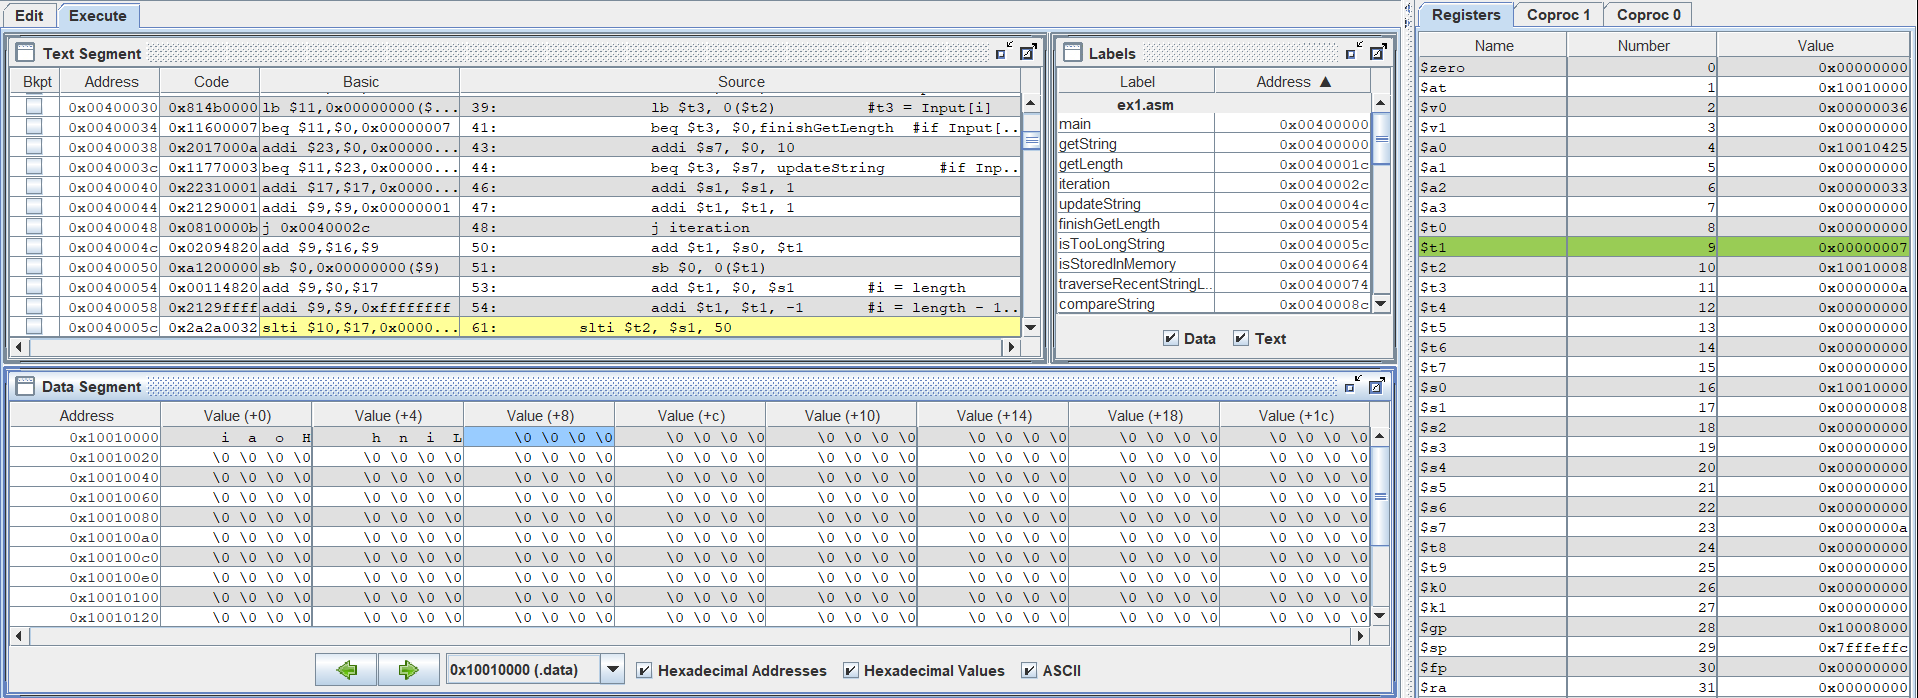
\includegraphics[width=1\textwidth]{bai1/L03-after-getLength.png}}}
	\caption{Kết quả sau khi thực hiện hàm getLength}
	\label{fig:bai1}
\end{figure}
\clearpage
\subsubsection{isTooLongString}
\begin{figure}[!h]
	\centerline{\fbox{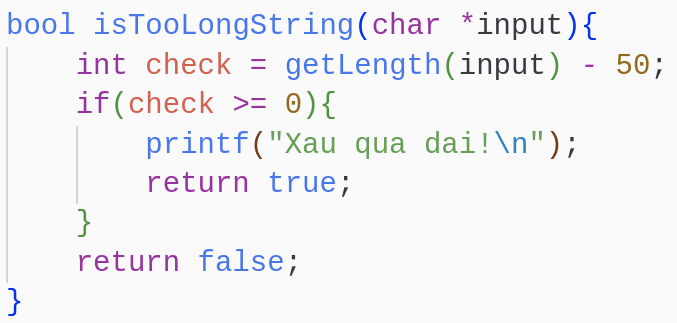
\includegraphics[width=1\textwidth]{bai1/1-toolong-c.png}}}
	\label{fig:bai6}
\end{figure}
\begin{figure}[!h]
	\centerline{\fbox{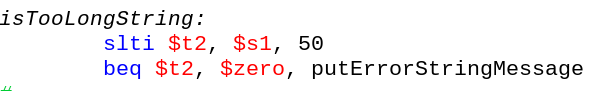
\includegraphics[width=1\textwidth]{bai1/1-toolong.png}}}
	\caption{Kiểm tra độ dài của xâu}
	\label{fig:bai6}
\end{figure}
% \clearpage
\noindent
\textbf{Trong đó: }
\begin{itemize}
    \item \$s1: Chỉ số i, dùng để chạy đến cuối xâu Input và lưu lại chỉ số của kí tự cuối cùng (tính từ 0).
    \item \$t2: Nếu độ dài của xâu Input (\$s1) < 50 thì \$t2 = 1, ngược lại \$t2 = 0.
\end{itemize}
\begin{figure}[!h]
	\centerline{\fbox{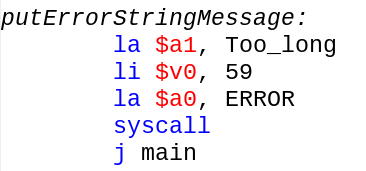
\includegraphics[width=1\textwidth]{bai1/1-putErrorStringMessage.png}}}
	\caption{Hàm thông báo lỗi quá kí tự cho phép}
	\label{fig:bai6}
\end{figure}
\noindent
\textbf{Giải thích: } 
Kiểm tra xem xâu nhập vào có dài quá 50 ký tự không (tính cả ký tự kết thúc xâu). Nếu dài hơn thì nhảy đến hàm \textbf{putErrorStringMessage} để in ra màn hình thông báo lỗi "Xau qua dai!". Sau đó hiển thị hộp thoại thông báo để người dùng nhập lại xâu..
\begin{figure}[!h]
	\centerline{\fbox{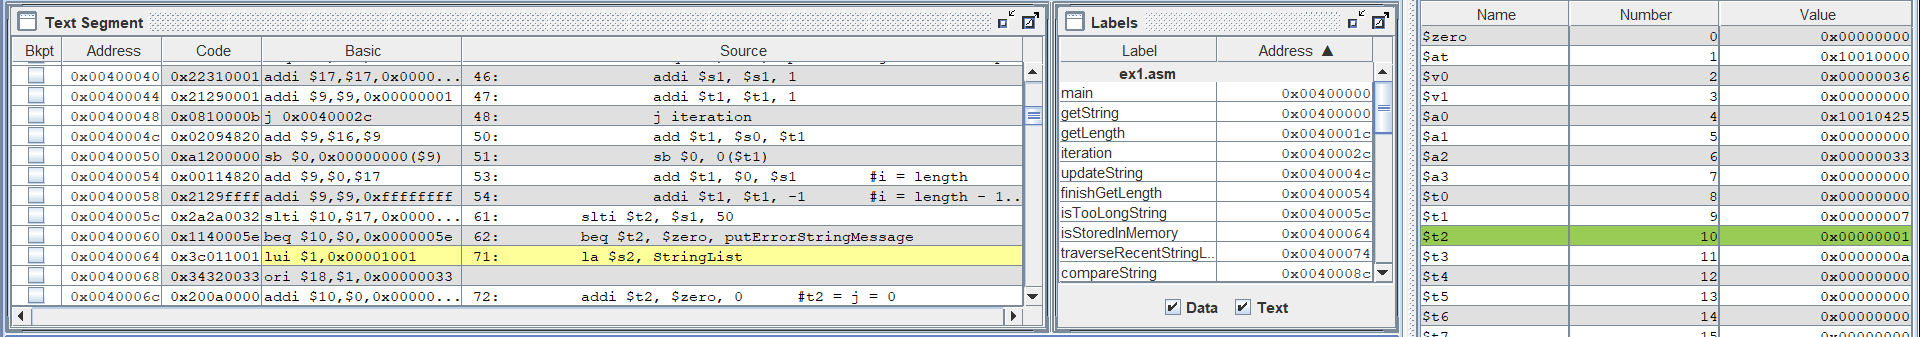
\includegraphics[width=1\textwidth]{bai1/L04-after-isTooLongString.png}}}
	\caption{Khi độ dài xâu thỏa mãn số lượng ký tự cho phép}
	\label{fig:bai1}
\end{figure}
\begin{figure}[!h]
	\centerline{\fbox{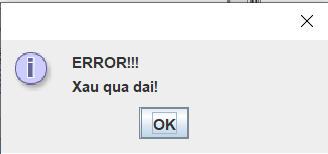
\includegraphics[width=1\textwidth]{bai1/L04-after-isTooLongString-error.png}}}
	\caption{Khi độ dài xâu vượt quá số lượng ký tự cho phép}
	\label{fig:bai1}
\end{figure}
\clearpage
\subsubsection{isStoredInMemory}
\begin{figure}[!h]
	\centerline{\fbox{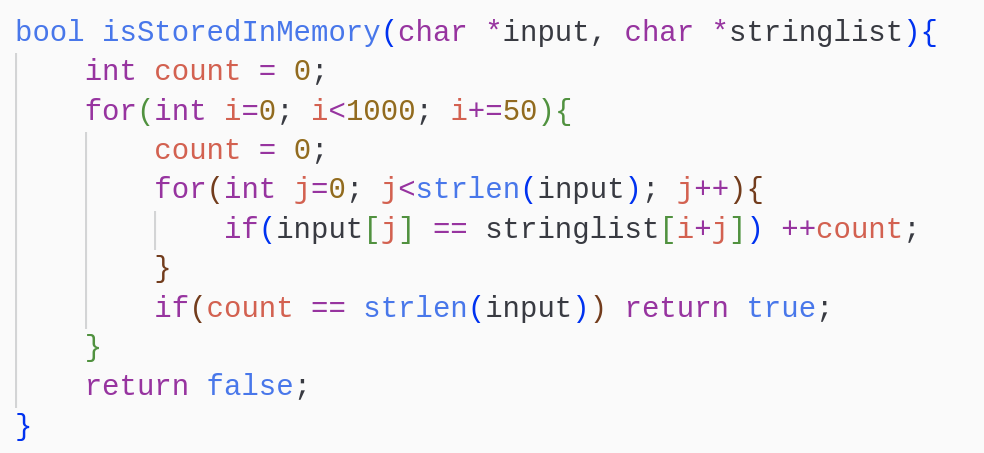
\includegraphics[width=0.85\textwidth]{bai1/1-isStoredInMemory-c.png}}}
	\label{fig:bai6}
\end{figure}
\begin{figure}[!h]
	\centerline{\fbox{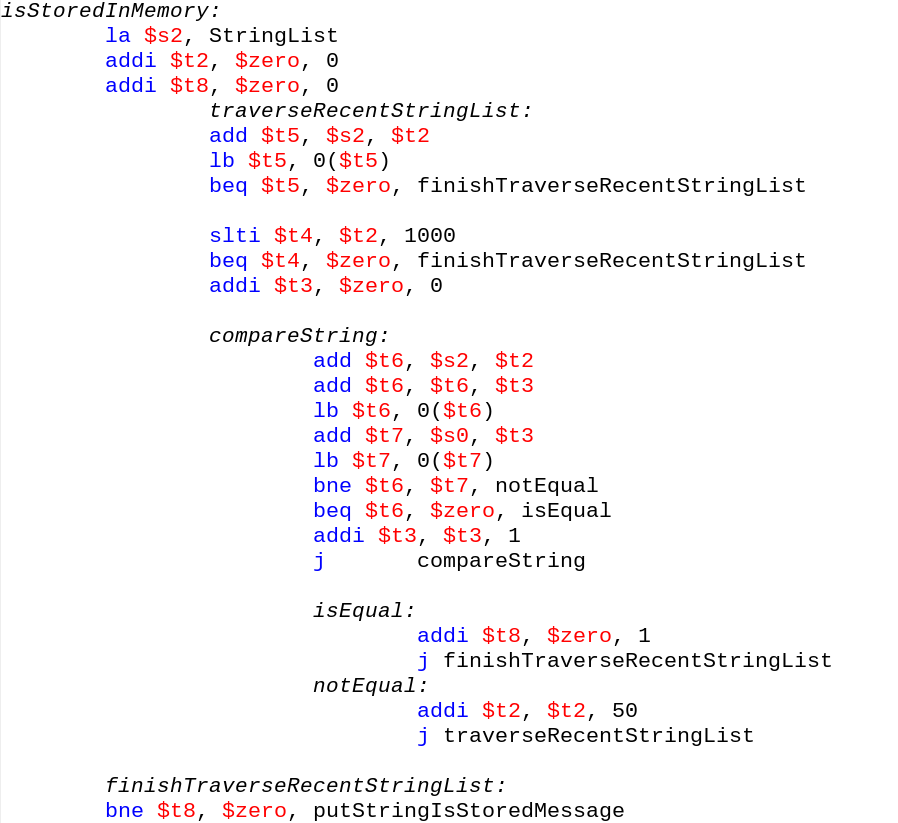
\includegraphics[width=0.85\textwidth]{bai1/1-isStoredInMemory.png}}}
	\caption{Hàm kiểm tra xâu đã lưu trong bộ nhớ}
	\label{fig:bai6}
\end{figure}
\clearpage
\noindent
\textbf{Trong đó: }
\begin{itemize}
    \item \$t2: Chỉ số j, dùng để chạy từ xâu đầu tiên đến xâu cuối cùng lưu trong mảng StringList với bước nhảy là 50 (do mỗi xâu trong mảng dài tối đa 50 ký tự).
    \item \$t3: Chỉ số k, dùng để chạy từ đầu đến cuối xâu Input.
    \item \$t4: Nếu chỉ số j đang xét (\$t2) < 1000 thì \$t4 = 1, tức là chưa duyệt hết mảng, ngược lại \$t4 = 0.
    \item \$t5: Lưu giá trị của phần tử thứ j trong mảng StringList.
    \item \$t6: Lưu giá trị của phần tử thứ j+k trong mảng StringList (StringList[j+k]).
    \item \$t7: Lưu giá trị của phần tử thứ k trong xâu Input (Input[k]).
    \item \$t8: Nếu xâu Input đã được lưu trong mảng StringList thì \$t8 nhận giá trị 1, ngược lại nhận giá trị 0.
\end{itemize}
\textbf{Giải thích: }
Ta duyệt từng xâu lưu trong mảng StringList bằng cách nhảy đến đầu mỗi xâu và kiểm tra xem nó có khác 0 hay không bằng cách dùng chỉ số j. Ta dừng duyệt khi phần tử StringList[j] = $'\backslash {0}'$ hoặc khi duyệt hết vùng nhớ dành cho mảng (1000 bits). \\
Mỗi khi duyệt một xâu, ta thực hiện so sánh xâu đó với xâu Input bằng cách so sánh từng phần tử của hai xâu lưu trong thanh ghi \$t6 và \$t7:
\begin{itemize}
    \item Nếu giá trị hai thanh ghi này không bằng nhau thì hai xâu khác nhau, ta tăng chỉ số j lên để tiếp tục kiểm tra xâu tiếp theo.
    \item Ngược lại, kiểm tra nếu giá trị thanh ghi \$t6 bằng 0 hay không, nếu có tức là hai xâu giống nhau từ đầu đến cuối xâu và xâu Input đã được lưu trong mảng, ta cập nhật \$t8 = 1, kết thúc duyệt, đưa thông báo ra màn hình và hỏi người dùng có muốn tiếp tục chương trình không.
\end{itemize}  
\begin{figure}[!h]
	\centerline{\fbox{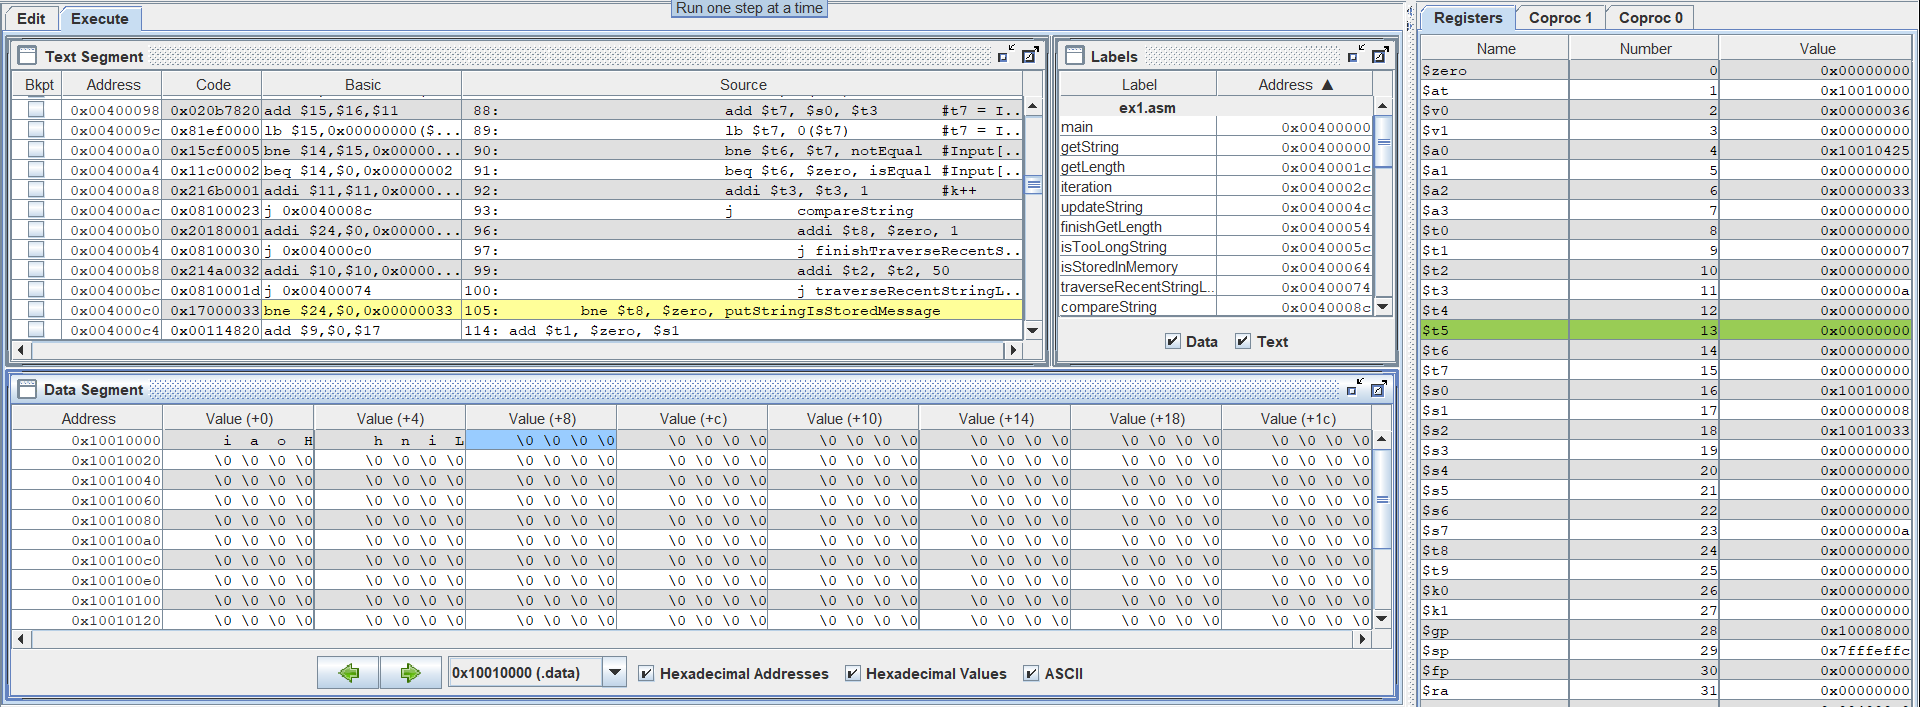
\includegraphics[width=1\textwidth]{bai1/L05-after-isStoredinMemory.png}}}
	\caption{Khi xâu chưa được lưu trong bộ nhớ, \$t8 = 0}
	\label{fig:bai1}
\end{figure}
\begin{figure}[!h]
	\centerline{\fbox{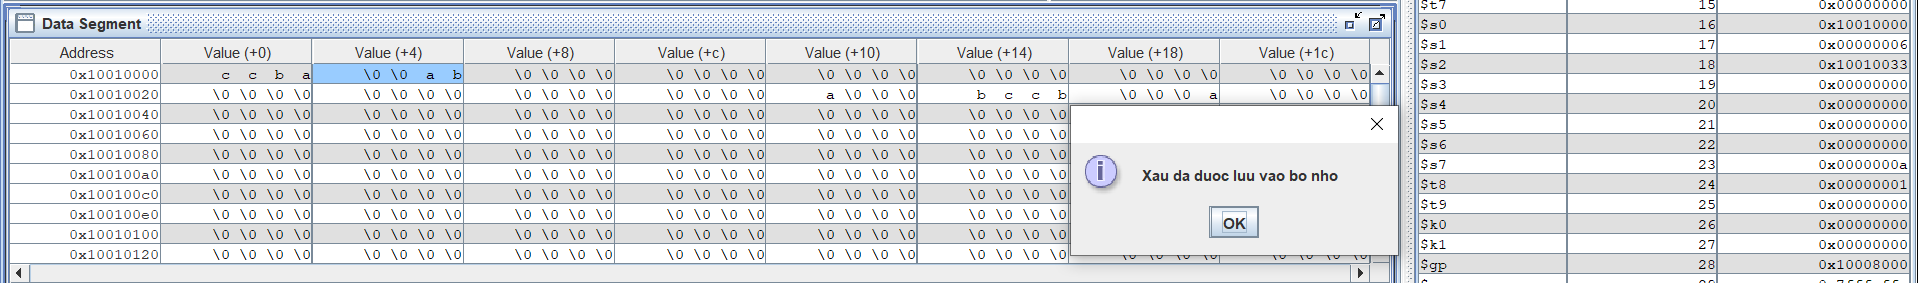
\includegraphics[width=1\textwidth]{bai1/L05-after-isStoredinMemory-error.png}}}
	\caption{Khi xâu đã được lưu trong bộ nhớ, \$t8 = 1 và thông báo}
	\label{fig:bai1}
\end{figure}
\clearpage
\subsubsection{checkPalindrome}
\begin{figure}[!h]
    \centerline{\fbox{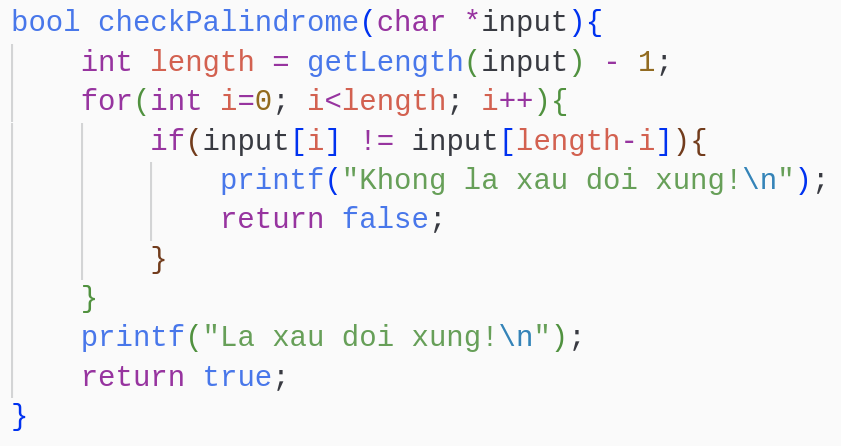
\includegraphics[width=0.75\textwidth]{bai1/1-checkPalindrome-c.png}}}
	\label{fig:bai6}
\end{figure}
% \clearpage
\begin{figure}[!h]
	\centerline{\fbox{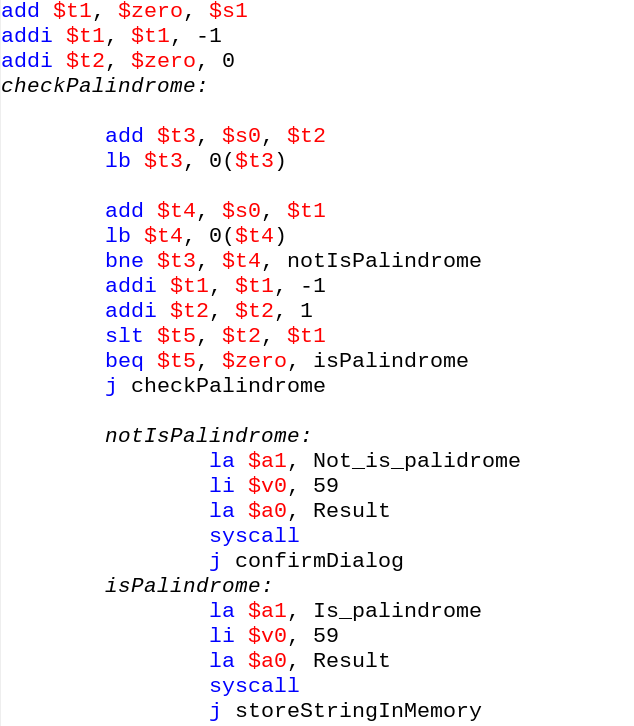
\includegraphics[width=0.75\textwidth]{bai1/1-checkPalindrome.png}}}
	\caption{Hàm kiểm tra đối xứng}
	\label{fig:bai6}
\end{figure}
\noindent
\textbf{Trong đó: }
\begin{itemize}
    \item \$t1: Chỉ số i, lưu lại chỉ số của kí tự cuối cùng (n-1), dùng để chạy từ cuối xâu Input lên đầu.
    \item \$t2: Chỉ số j, chạy từ đầu xâu Input về cuối.
    \item \$t3: Lưu giá trị của phần tử thứ j trong xâu Input (Input[j]).
    \item \$t4: Lưu giá trị của phần tử thứ i trong xâu Input (Input[i]).
    \item \$t5: Nếu chỉ số j < i thì \$t5 nhận giá trị 1, ngược lại nhận giá trị 0.
\end{itemize}
\textbf{Giải thích: } 
So sánh lần lượt các phần tử ở phần đầu (chỉ số j) và ở phần cuối xâu (chỉ số i) theo thứ tự (Input[0] với Input[n-1], (Input[1] với Input[n-2]...) Nếu có một cặp khác nhau thì xâu không đối xứng. Nếu không thì kiểm tra cho đến j < i thì dừng lại, khi đó xâu là đối xứng.  \\
Sau khi kiểm tra, ta in kết quả ra màn hình và hỏi người dùng có muốn tiếp tục chương trình nếu xâu không đối xứng hoặc lưu xâu vừa nhập nếu đó là xâu đối xứng.
\clearpage
\noindent
\textbf{Kết quả kiểm tra:}
\begin{figure}[!h]
	\centerline{\fbox{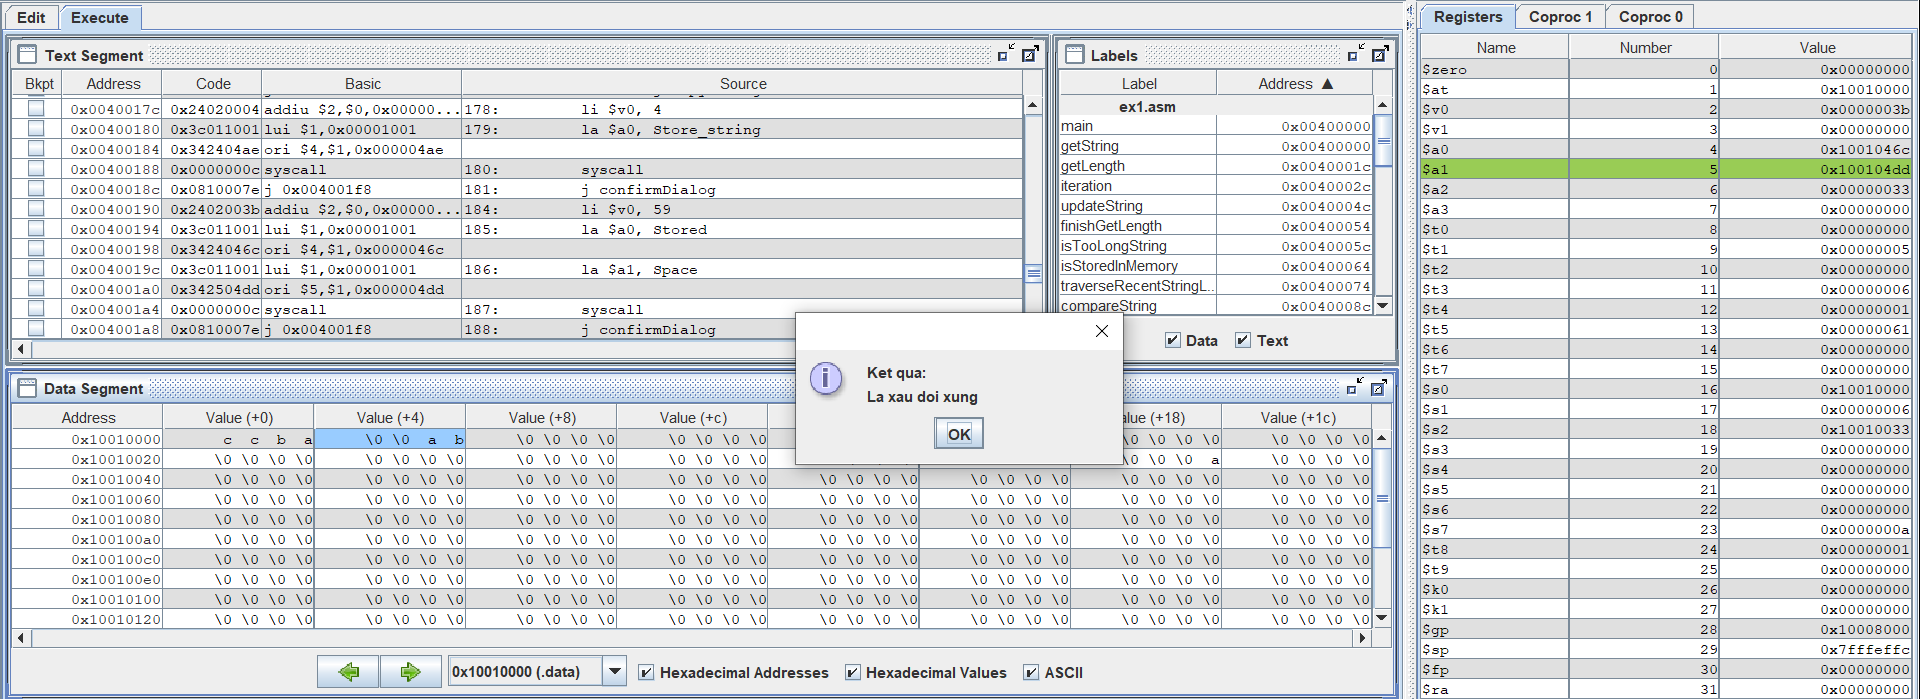
\includegraphics[width=1\textwidth]{bai1/L06-after-checkPalindrome-1.png}}}
	\caption{Khi xâu đối xứng}
	\label{fig:bai6}
\end{figure}
\begin{figure}[!h]
	\centerline{\fbox{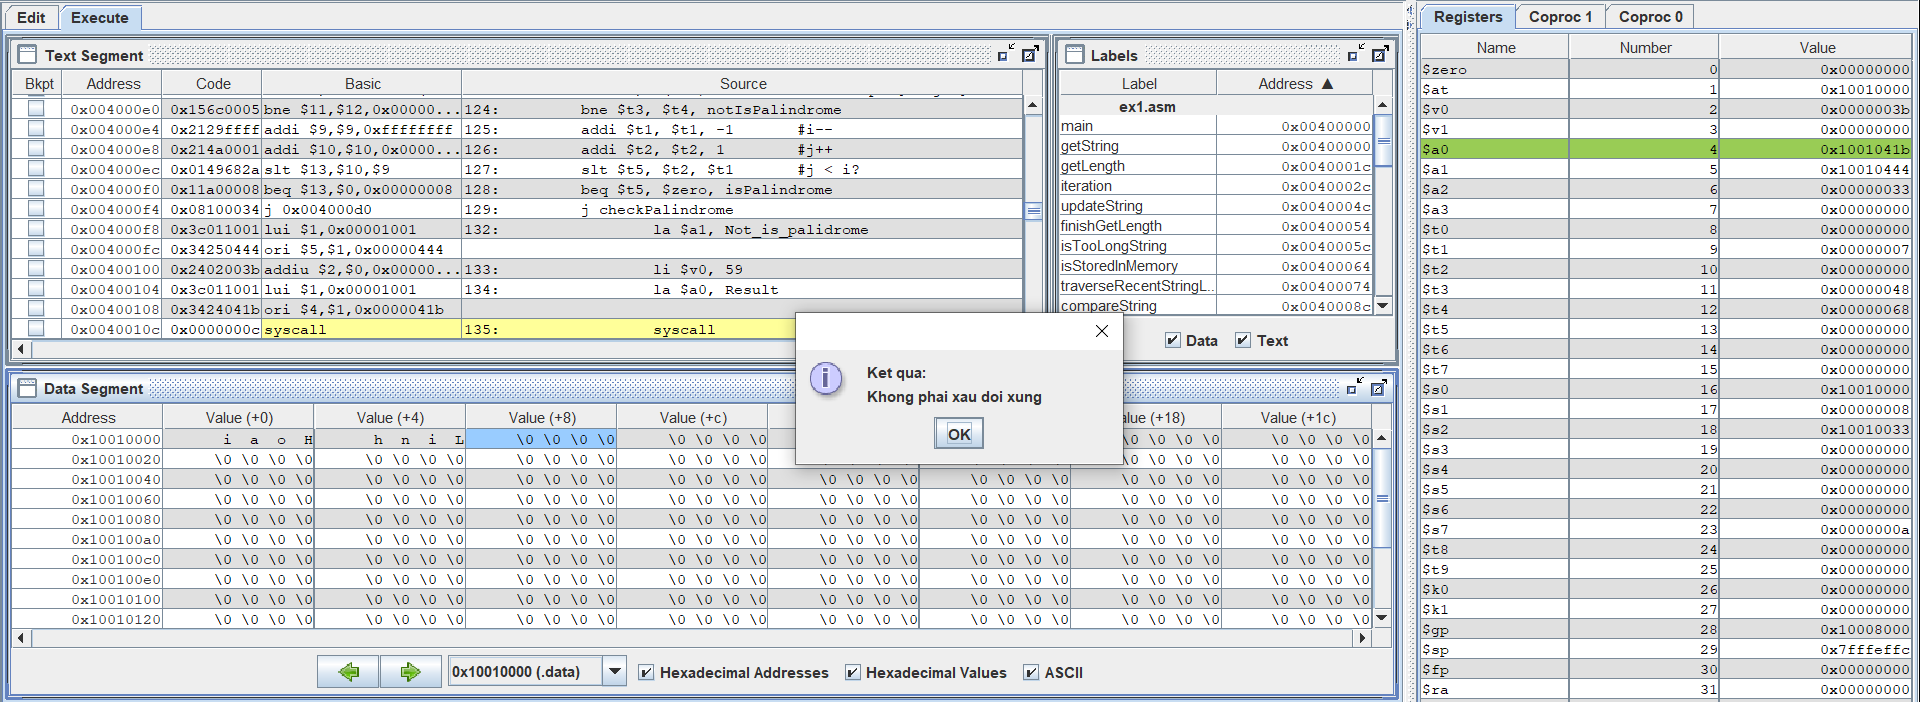
\includegraphics[width=1\textwidth]{bai1/L06-after-checkPalindrome-2.png}}}
	\caption{Khi xâu không đối xứng}
	\label{fig:bai6}
\end{figure}
\clearpage
\subsubsection{storeStringInMemory}
\begin{figure}[!h]
    \centerline{\fbox{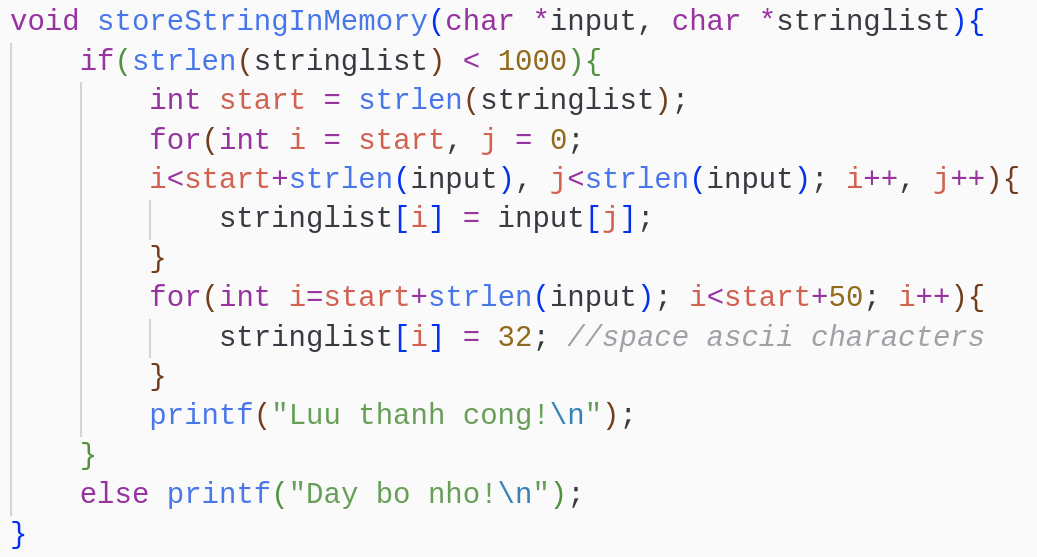
\includegraphics[width=0.9\textwidth]{bai1/1-storeStringInMemory-c.png}}}
	\label{fig:bai6}
\end{figure}
\begin{figure}[!h]
	\centerline{\fbox{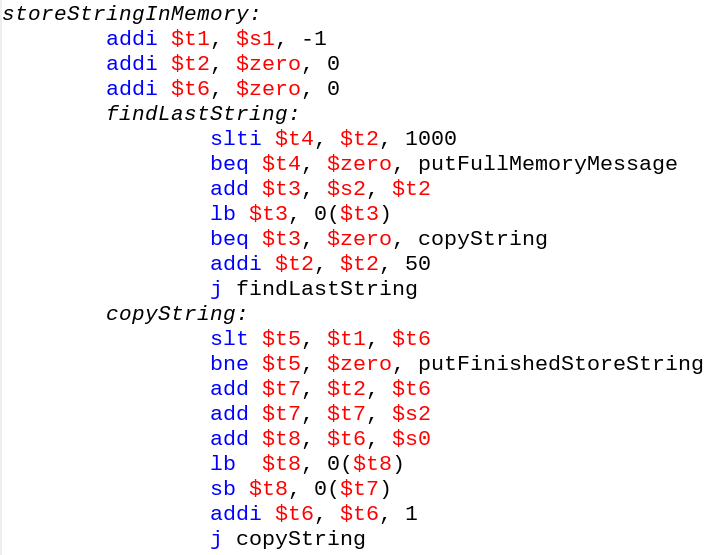
\includegraphics[width=0.9\textwidth]{bai1/1-storeStringInMemory.png}}}
	\caption{Hàm lưu xâu đối xứng vào bộ nhớ}
	\label{fig:bai6}
\end{figure}
\noindent
\clearpage
\textbf{Trong đó: }
\begin{itemize}
    \item \$t1: Chỉ số i, lưu lại chỉ số của kí tự cuối cùng (n-1).
    \item \$t2: Chỉ số j, dùng để chạy từ xâu đầu tiên đến xâu cuối cùng lưu trong mảng StringList với bước nhảy là 50 (do mỗi xâu trong mảng dài tối đa 50 ký tự).
    \item \$t3: Lưu giá trị của phần tử thứ j trong mảng StringList.
    \item \$t4: Nếu chỉ số j đang xét (\$t2) < 1000 thì \$t4 = 1, tức là chưa duyệt hết mảng, ngược lại \$t4 = 0.
    \item \$t5: Nếu chỉ số i < j, tức là đã lưu hết xâu, thì \$t5 nhận giá trị 1, ngược lại nhận giá trị 0.
    \item \$t6: Chỉ số k, dùng để chạy từ đầu đến cuối xâu Input.
    \item \$t7: Địa chỉ của phần tử thứ j+k trong mảng StringList (StringList[j+k]).
    \item \$t8: Lưu giá trị của phần tử thứ k trong xâu Input (Input[k]).
\end{itemize}
\textbf{Giải thích: } 
Đầu tiên, ta tìm vị trí trống ngay sau xâu cuối cùng đã lưu trong mảng, tương tự như ở hàm kiểm tra xâu đã lưu trong bộ nhớ. Ta duyệt từng xâu lưu trong mảng StringList bằng cách nhảy đến đầu mỗi xâu và kiểm tra xem nó có khác 0 hay không. Ta dừng duyệt khi duyệt hết vùng nhớ dành cho mảng (1000 bits) hoặc khi thấy phần tử StringList[j] = $'\backslash {0}'$.
\begin{itemize}
    \item Nếu bộ nhớ đầy ta đưa thông báo ra màn hình rồi hỏi người dùng có muốn tiếp tục chương trình không.
    \item Nếu tìm thấy vị trí trống, ta thực hiện hàm \textbf{copyString} để lưu xâu vừa nhập vào bộ nhớ. Lần lượt lấy từng giá trị của phần tử trong xâu Input (\$t8) lưu vào địa chỉ tương ứng trong bộ nhớ (\$t7) cho đến khi chỉ số j tăng đến lớn hơn i = n - 1 thì kết thúc. Ta chuyển đến hàm \textbf{putFinishStoreString} để in ra thông báo và sau đó hỏi người dùng có muốn tiếp tục chương trình không.
\end{itemize}  
\clearpage
\noindent
\textbf{Kết quả:} Các xâu đối xứng được lưu vào bộ nhớ bắt đầu từ địa chỉ 0x10010033 theo đúng địa chỉ đã được cấp phát ban đầu.
\begin{figure}[!h]
	\centerline{\fbox{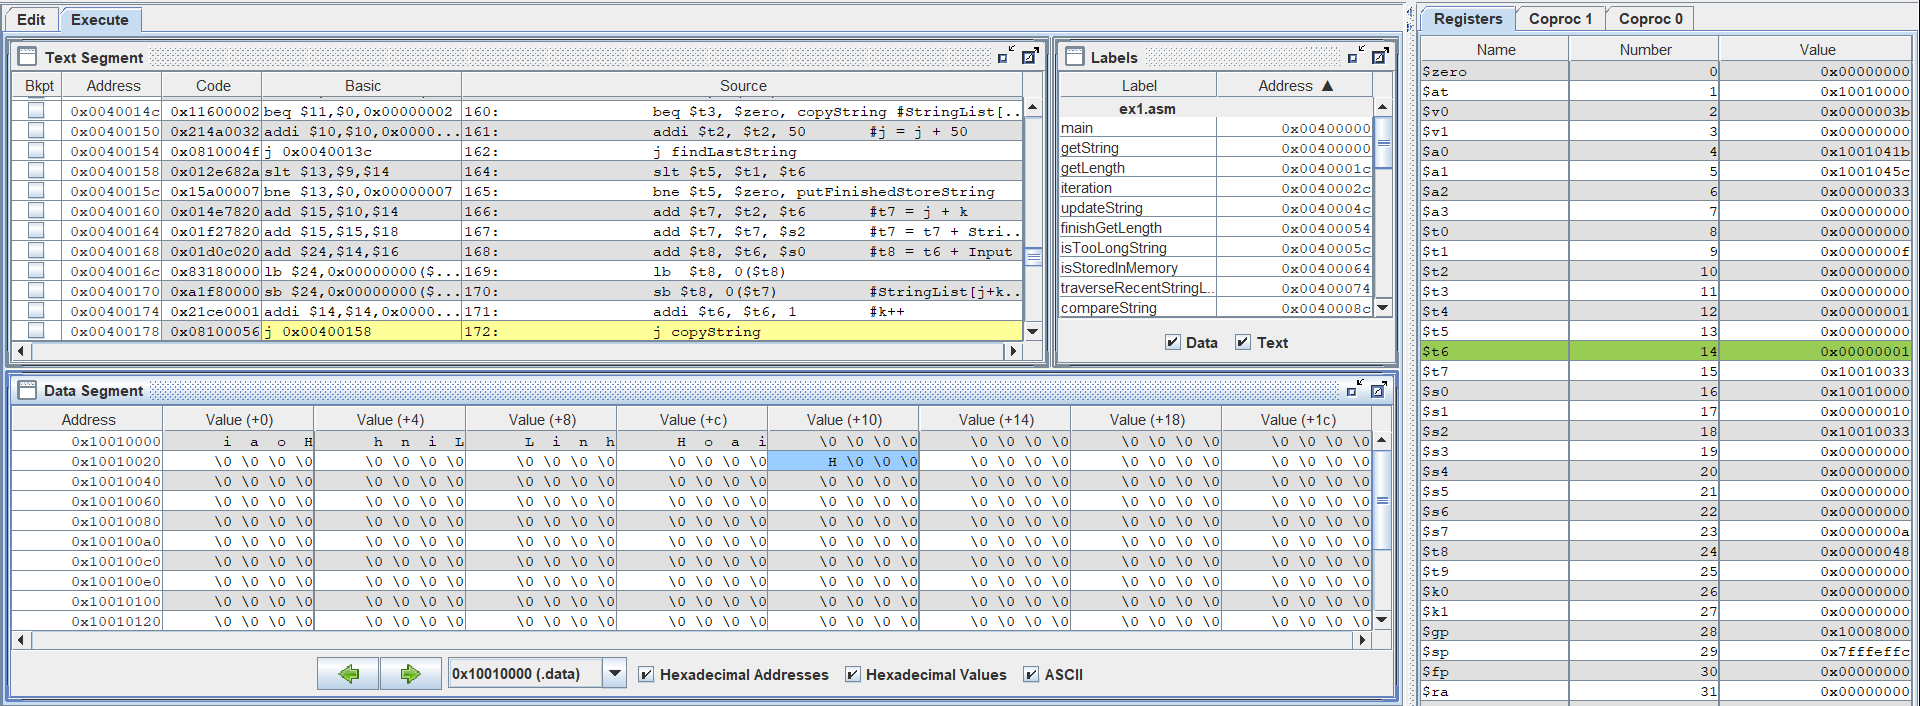
\includegraphics[width=0.75\textwidth]{bai1/L14-stored-byte-1.png}}}
	\caption{Bộ nhớ sau khi lưu ký tự đầu tiên vào bộ nhớ}
	\label{fig:bai6}
\end{figure}
\begin{figure}[!h]
	\centerline{\fbox{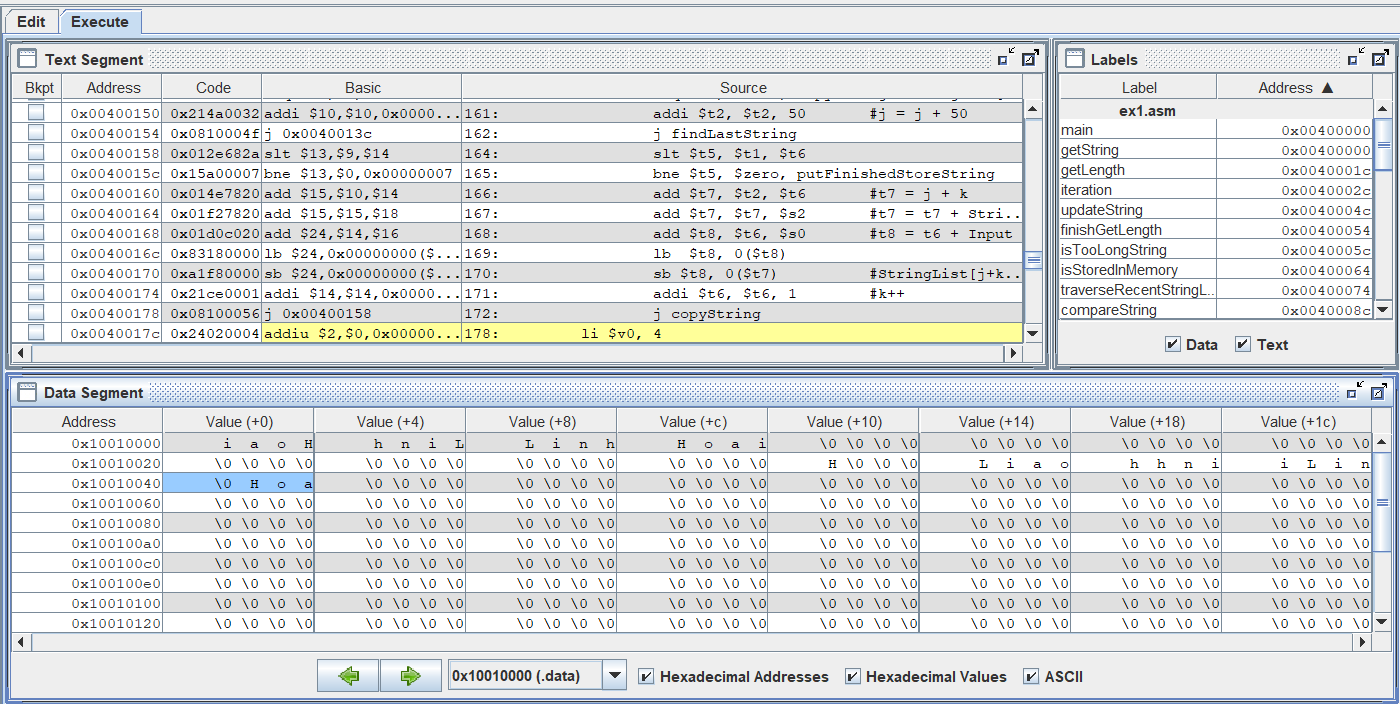
\includegraphics[width=0.75\textwidth]{bai1/L15-after-StoredinMemory.png}}}
	\caption{Bộ nhớ sau khi lưu một xâu}
	\label{fig:bai6}
\end{figure}
\begin{figure}[!h]
	\centerline{\fbox{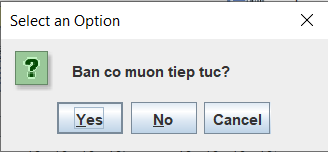
\includegraphics[width=0.75\textwidth]{bai1/L07-confirm-dialog.png}}}
	\caption{Hộp thoại xác nhận tiếp tục chương trình}
	\label{fig:bai6}
\end{figure}
\end{document}